\documentclass[a4j]{jarticle}
%%  packages
\usepackage{amsmath,amssymb,ascmac}
\usepackage{bm}
\usepackage[dvipdfmx]{graphicx}
\usepackage{listings}
\usepackage[english]{babel}
\lstset{
 	%枠外に行った時の自動改行
 	breaklines = true,
 	%標準の書体
        basicstyle=\ttfamily\footnotesize,
        commentstyle=\footnotesize\bfseries,
        keywordstyle=\footnotesize\bfseries,
 	%枠 "t"は上に線を記載, "T"は上に二重線を記載
	%他オプション:leftline,topline,bottomline,lines,single,shadowbox
 	frame = single,
 	%frameまでの間隔(行番号とプログラムの間)
 	framesep = 5pt,
 	%行番号の位置
 	numbers = left,
	%行番号の間隔
 	stepnumber = 1,
	%タブの大きさ
 	tabsize = 4,
 	%キャプションの場所("tb"ならば上下両方に記載)
 	captionpos = t
}

%% math commands
\let \ds \displaystyle
\newcommand{\idiff}[3]{
  \frac{d^{#1} #2}{d #3^{#1}}
}
\newcommand{\diff}[3]{
  \frac{\mathrm{d}^{#1} #2}{\mathrm{d} #3^{#1}}
}
\newcommand{\pdiff}[3]{
  \frac{\partial^{#1} #2}{\partial #3^{#1}}
}



%% title configuration
\title{計算アルゴリズムレポート(課題1)}
\author{05-161026(情報科学科) 平出一郎}
\date{\today}


%% headings
\pagestyle{headings}
\markright{}




\begin{document}
%%  begin title page
\thispagestyle{empty}
\maketitle
\pagebreak


%% begin contents


二次元正方領域上でのポアソン方程式を差分法で解いた。


解析解として$\ds u=\sin(2\pi x)\sin(2\pi y)$を用いた。このとき$\ds - \left( \pdiff{2}{u}{x}+\pdiff{2}{u}{y} \right)= f(x,y) = 8\pi^2\sin(2\pi x)\sin(2\pi y)$となり、これを境界上でのDirichlet条件の下で解く。


このとき離散化された方程式は各$i,j$に対して、$$\ds - \left( \frac{u_{i+1,j}-2u_{i,j}+u_{i-1,j}}{(\Delta x)^2}+\frac{u_{i,j+1}-2u_{i,j}+u_{i,j-1}}{(\Delta y)^2} \right) = f(x_i,y_j)$$で表される。


これを$\ds {\bm u} = (u_{1,1}\hspace{2mm}u_{1,2}\hspace{2mm}\cdots\hspace{2mm}u_{n-1,n-2}\hspace{2mm}u_{n-1,n-1})^\top$と書いた時に$A{\bm u}={\bm b}$の連立方程式の形で書き表すと$A$は対称行列となる。これをCG法で解く。

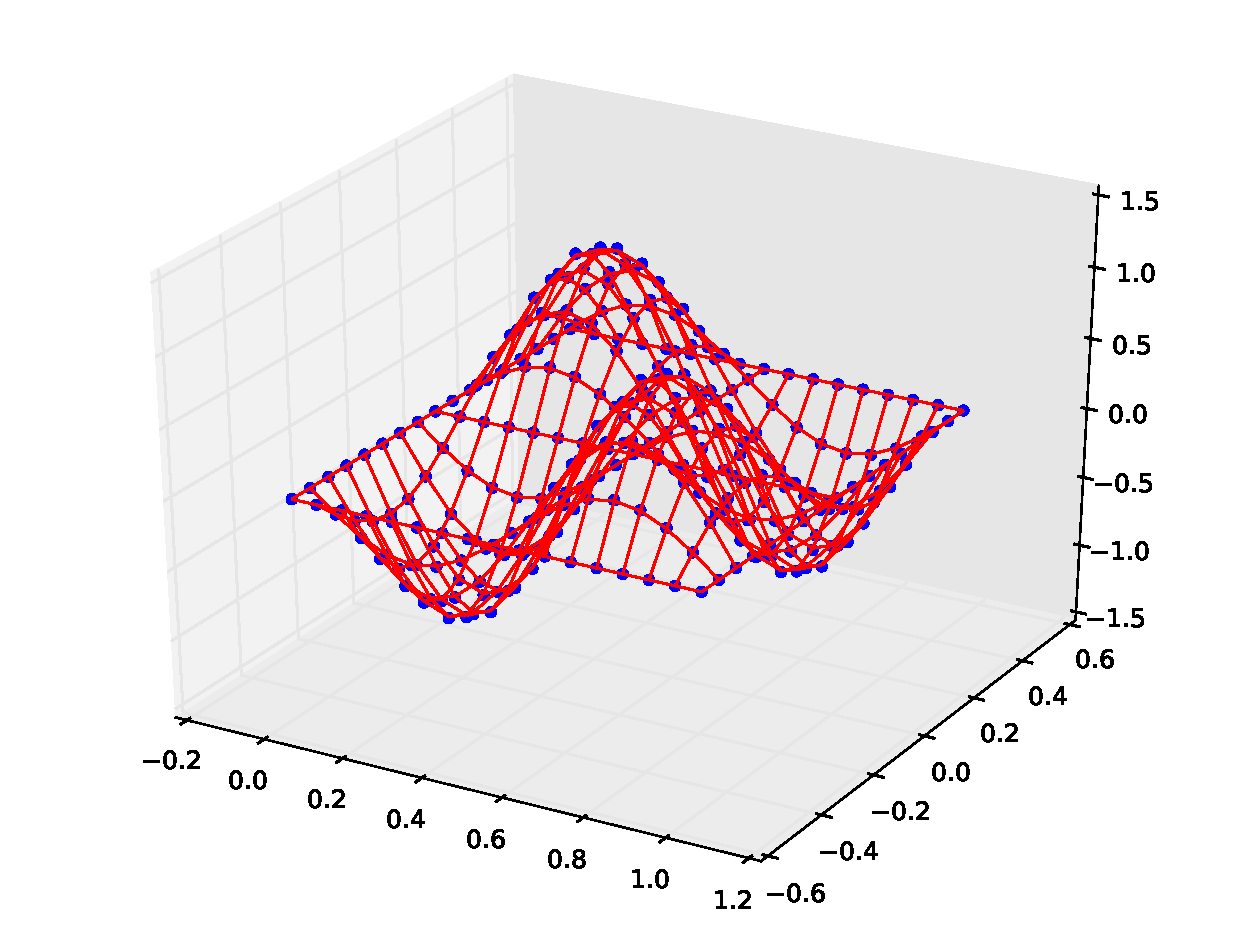
\includegraphics[width=7cm]{3D.eps}


赤が解析解からプロットしたメッシュで、青が離散化した方程式の解である。解析解を近似できていることが確認できる。


プログラムはpythonで記述しソースコードをレポートの末尾に記載した。任意の矩形領域と分割数、及びDirichlet条件下での任意の$u,f$に対応するようにした。scipy.sparseから疎行列を用いることで、より大きい分割数でも計算が可能となるようにした。



\section{差分の刻み幅と反復回数との関係を調べよ}

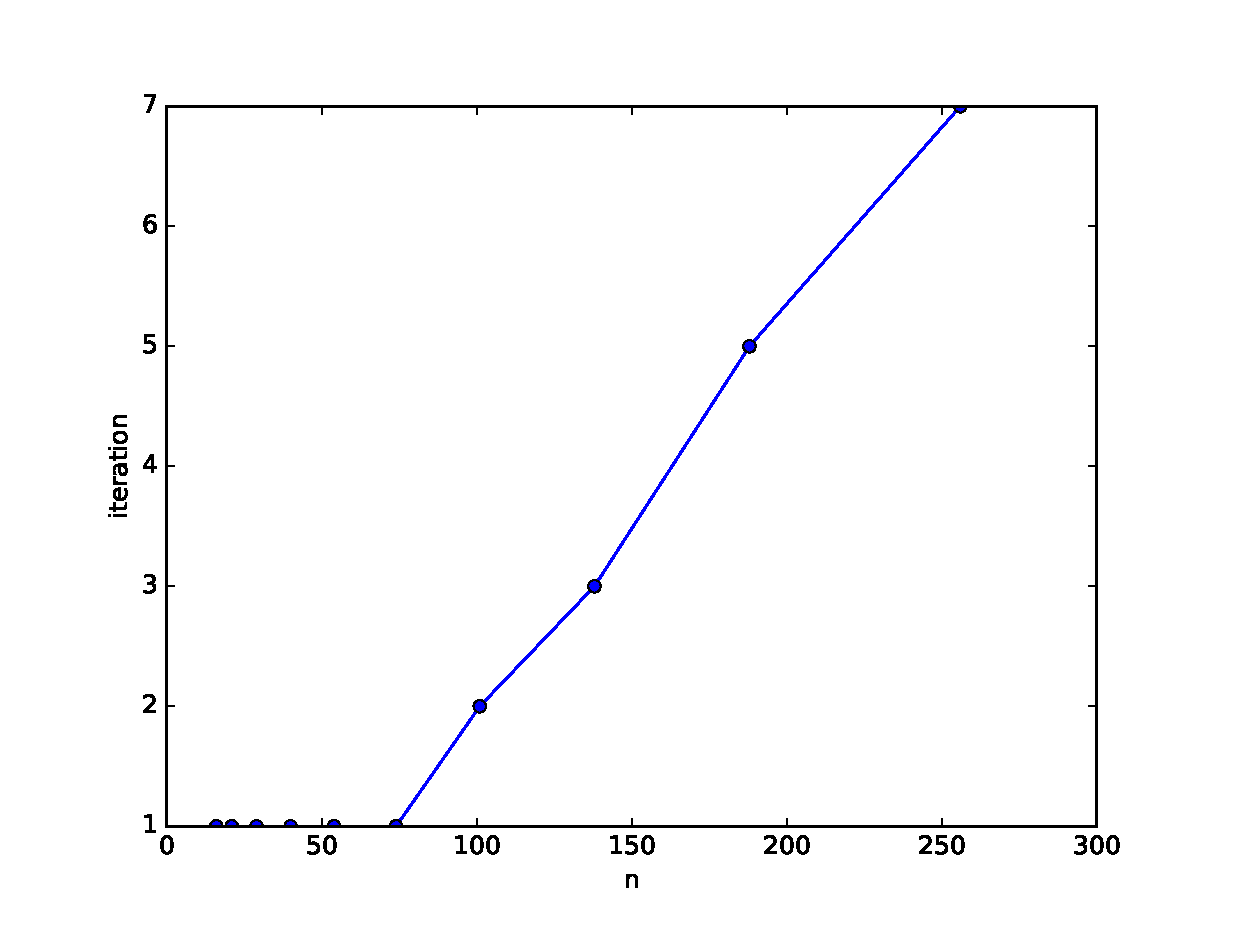
\includegraphics[width=7cm]{iteration.eps}


グラフから、分割数を増加させるとCG法の反復回数は線形に増加していることがわかる。ただし、分割数が少ないと1回で収束することもありうることがわかる。

\section{離散化の精度を上げた時の適合性・収束性を確認せよ}


\section{両対数グラフに刻み幅と誤差ノルムをプロットして収束の速さを実験的に評価せよ}


$\tilde{\bm u}$を厳密解$u(x_i,y_j)$を並べたベクトルとする。適合性の尺度として$ \left\| {\bm b} - A\tilde{\bm u} \right\|_\infty$、収束性の尺度として$\left\| {\bm u}-\tilde{\bm u} \right\|_\infty$を求めた。両対数グラフに横軸を刻み幅$h$を用いてプロットした。


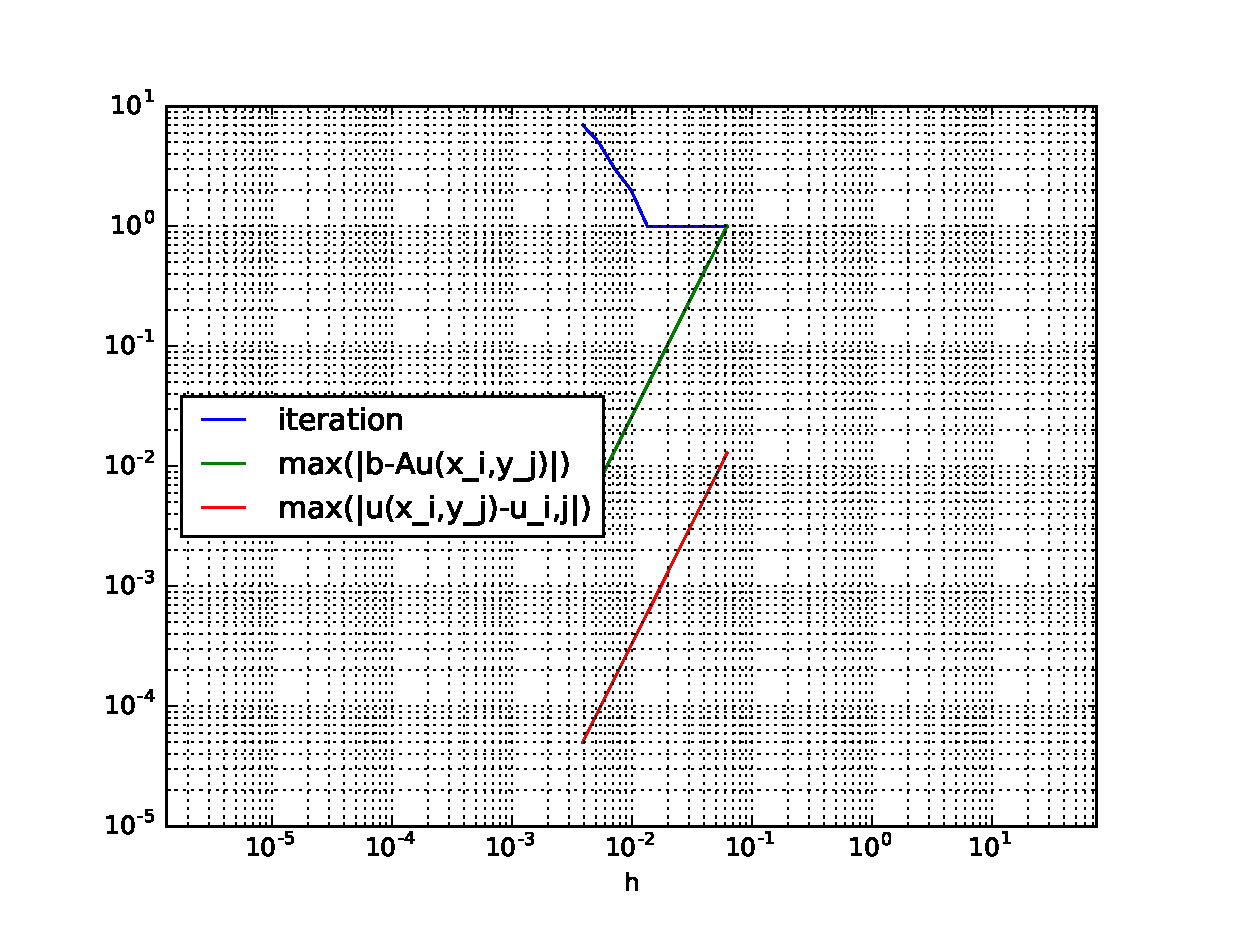
\includegraphics[width=7cm]{loglog.eps}

$ \left\| {\bm b} - A\tilde{\bm u} \right\|_\infty$,$\left\| {\bm u}-\tilde{\bm u} \right\|_\infty$は刻み幅を小さくすると減少することが確認できる。また、グラフの傾きから刻み幅に対して二次収束することが確認できる。これは2階中央差分がテイラー展開の二次項まで一致することに対応している。

\section{ソースコード}


\lstinputlisting[language=python]{main.py}

\end{document}


